\documentclass[11pt]{article}
\usepackage{amsmath, color, graphicx, indentfirst, float, wrapfig, siunitx}
\usepackage[margin=1in]{geometry}

\title{Computational Physics: Homework 1 }
\author{Austin McDowell}
\date{}
\begin{document}
\maketitle

\section*{Problem 1}
\subsection*{Introduction}
In this problem we created a plot of the Mandelbrot set. The Mandelbrot set created iteratively using the equation
\begin{equation}
\label{eq:man_eq}
z^\prime = z^2 + c
\end{equation}
where $z$ is a complex input number and $c = x + iy$ is another complex number used to create the output, $z^\prime$. For a pair of $x$ and $y$ values we create the complex number $c$ and start with $z=0$. We then iterate using equation (\ref{eq:man_eq}) and if $|z|>2$ then the point at $(x,y)$ is \textbf{not} in the Mandelbrot set. 

\subsection*{Methods}
For our purposes we made a evenly spaced grid in $x$ and $y$ ranging from -2 to 2 with which the values for $c$ were made. For each point, we iterated a maximum of 100 times to check if the point at $(x,y)$ was in the set. At first our grid size was 100x100 but it was ultimately increased to 750x750 to produce the final plots.

To keep track of whether an $(x,y)$ pair was in the set, an array of zeros, $Z$, of size $(N,N)$ was created where $N$ is the size of the $x$ and $y$ grids. If, $|z|$ was ever greater than 2, the corresponding point in $Z$ was left as 0. If, after 100 iterations, the value for $|z|$ was less than 2, the corresponding point was given a value of 1. This method was used to make a 'binary' Mandelbrot set where points are considered either 'in' or 'out'. Additionally, a Mandelbrot 'density' plot was made where the value in $Z$ was incremented based on the number of iterations before $|z|$ becomes larger than 2. 

\subsection*{Results}
The generated Mandelbrot figures are shown below. The black and white figure is the binary plot where black indicates points included in the set. The density plot is shown in Figure 2 with redder colors indicating increasing iterations. 


\begin{figure}[H]
  \centering
  \begin{minipage}[t]{0.4\textwidth}
    \centering
    \vspace{0pt}
    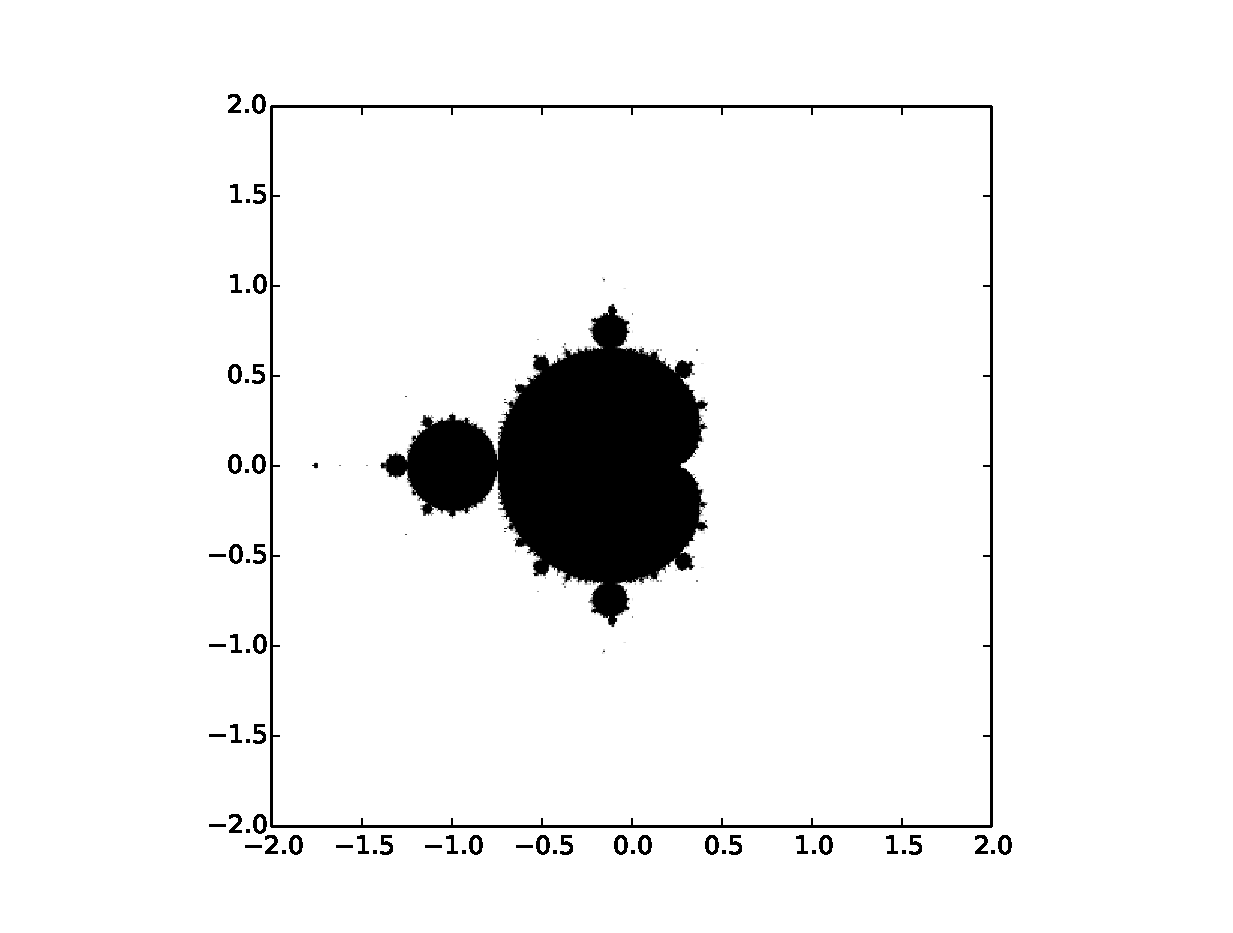
\includegraphics[scale=0.42]{mandel_1.eps}
    \caption{\scriptsize Binary Mandelbrot plot}
  \end{minipage} \hfill
  \begin{minipage}[t]{0.4\textwidth}
    \centering
    \vspace{0pt}
    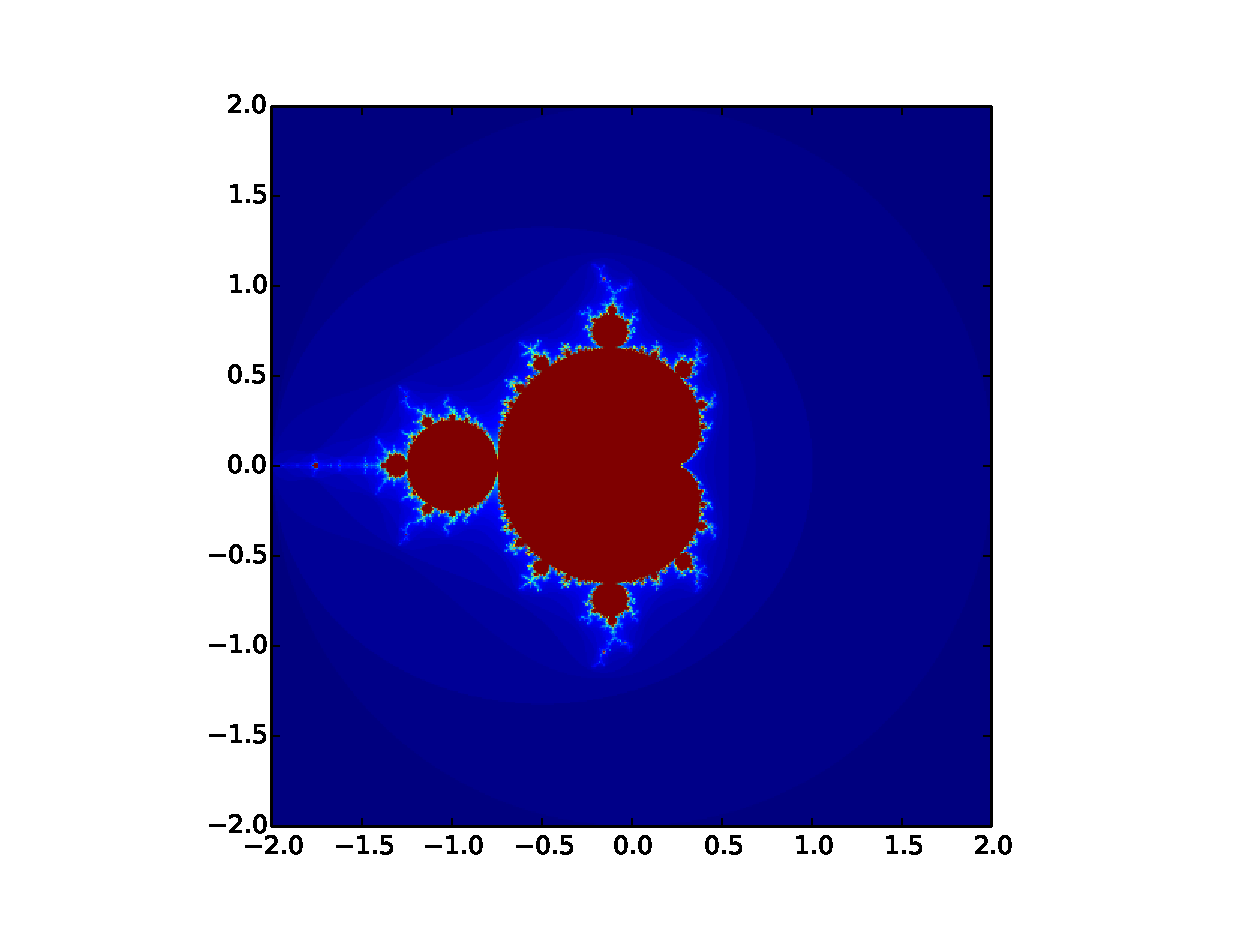
\includegraphics[scale=0.42]{mandel_2.eps}
    \caption{\scriptsize Mandelbrot density plot}
  \end{minipage}
\end{figure}


\section*{Problem 2}
\subsection*{Introduction}
In this problem we wrote our own linear least squares fitting code to fit data from the Millikan oil drop experiment and calculate a value for Planck's constant, $h$. 

For a given set of points, a linear least squares fit determines the equation of a line that minimizes the square of the distance between the points and the line. Suppose we have a line given by $y=mx+c$ where $m$ is the slope and $c$ is the y-intercept, the distance, $d$,  between the line and a point $(x_i, y_i)$ is given by
\begin{displaymath}
d = mx_i + c - y_i
\end{displaymath} 
For $N$ points, the sum of the square of all these distances, $\chi^2$, is given by
\begin{equation}
\chi^2 = \sum_{i=1}^N (mx_i + c - y_i)^2.
\end{equation}
The method of linear least squares minimizes this sum with respect to $m$ and $c$ to find the best fit line. By taking the derivative of $\chi^2$ with respect to $m$ and $c$ and setting them equal to zero, it can be shown that $m$ and $c$ can be expressed as
\begin{equation}
\label{eq:m}
m = \frac{ E_{xy} - E_x E_y }{ E_{xx} - E_x^2}
\end{equation}
and
\begin{equation}
\label{eq:m}
c = \frac{ E_{xx}E_y - E_x E_{xy} }{ E_{xx} - E_x^2}
\end{equation}
where 
\begin{displaymath}
E_x = \frac{1}{N} \sum_{i=1}^N x_i \quad\mathrm{;}\quad E_y = \frac{1}{N} \sum_{i=1}^N y_i \quad\mathrm{;}\quad E_{xx} = \frac{1}{N} \sum_{i=1}^N x_i^2 \quad\mathrm{;}\quad E_{xy} = \frac{1}{N} \sum_{i=1}^N x_i y_i
\end{displaymath}
 
\subsection*{Methods}
With the data provided in \texttt{millikan.txt} and the above equations, we first solved for the parameters of the line, $m$ and $c$. The data should be described by the equation for the voltage of a conduction electron ejected by a photon with frequency $\nu$
\begin{displaymath}
V = \frac{h}{e}\nu - \phi
\end{displaymath} 
where $e$ is the charge of an electron and $\phi$ is the 'work function' or energy needed to eject an electron from a metal surface. We know the charge of an electron so if we fit this data to a line, we can solve for $h$ using $h = m * e$. 
\subsection*{Results}
A plot of the Millikan data and the best fit line is shown below. 
\begin{figure}[H]
  \centering
  \begin{minipage}[t]{0.5\textwidth}
    \centering
    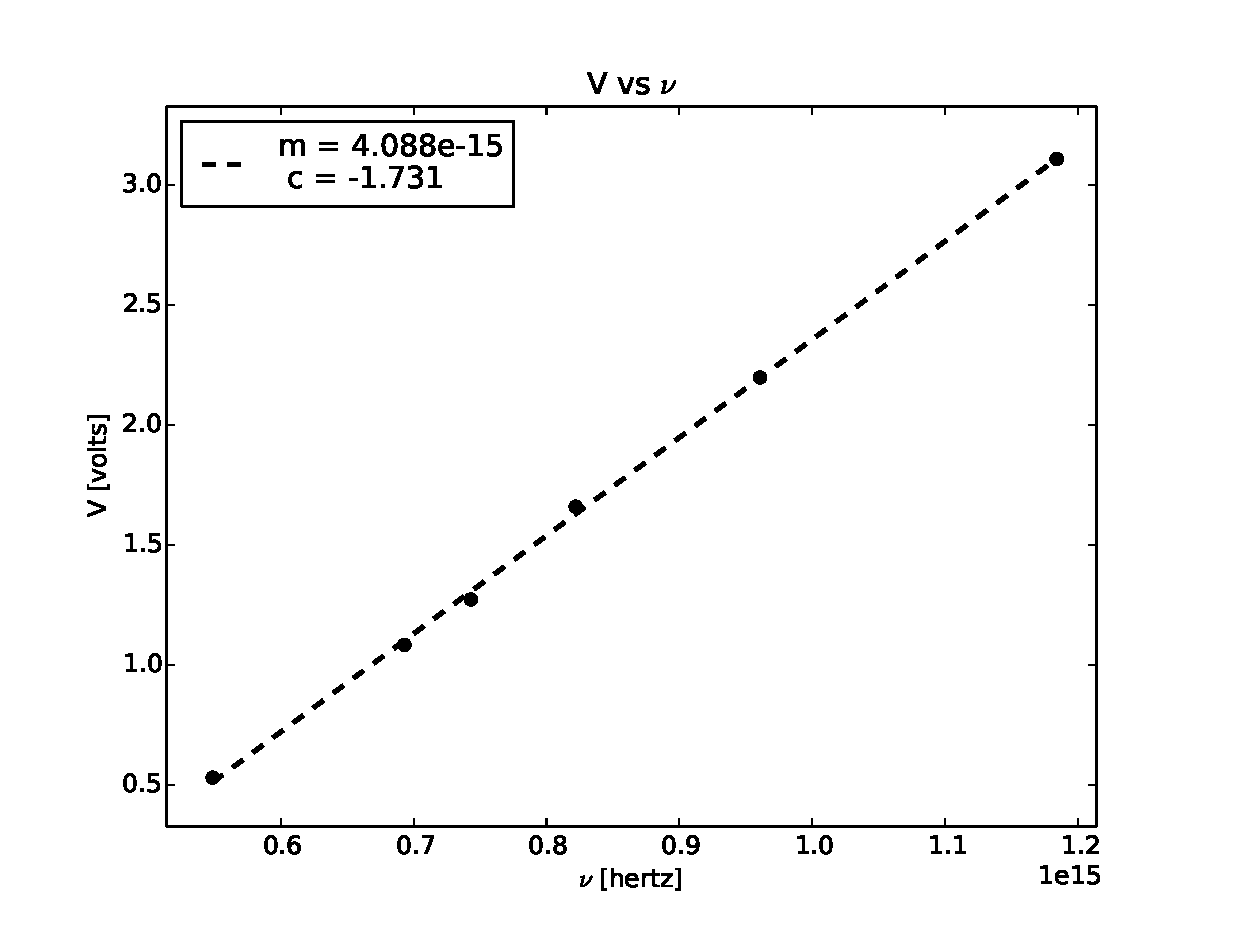
\includegraphics[width=\linewidth]{milli.eps}
    \caption{\scriptsize Millikan data and best fit line found using linear least squares. Slope and y-intercept are listed in the top left }
    \label{fig:elevels}
   \end{minipage}
\end{figure}
Using the value of the slope and $e=1.602 \times 10^{-19} C$, the value for Planck's constant was found to be
\begin{displaymath}
\boxed{ h = 6.549 \times 10^{-34} \tagaddtext{[\si{\meter\squared\kilogram\per\s\squared}]}}
\end{displaymath}
which is within $1.2\%$ of the accepted value. 


\end{document}
